% Created 2025-06-05 Thu 20:54
% Intended LaTeX compiler: pdflatex
\documentclass[11pt]{article}
\usepackage[utf8]{inputenc}
\usepackage[T1]{fontenc}
\usepackage{graphicx}
\usepackage{longtable}
\usepackage{wrapfig}
\usepackage{rotating}
\usepackage[normalem]{ulem}
\usepackage{amsmath}
\usepackage{amssymb}
\usepackage{capt-of}
\usepackage{hyperref}
\usepackage{minted}
\usepackage[polski, polish]{babel}
\author{Michał Kamiński, \textbf{Mikołaj Szustakowski}, Nikodem Rękiewicz, Szymon Mastalerz}
\date{\today}
\title{CADR}
\hypersetup{
 pdfauthor={Michał Kamiński, \textbf{Mikołaj Szustakowski}, Nikodem Rękiewicz, Szymon Mastalerz},
 pdftitle={CADR},
 pdfkeywords={},
 pdfsubject={},
 pdfcreator={Emacs 30.1 (Org mode 9.7.30)}, 
 pdflang={Polish}}
\begin{document}

\maketitle
\tableofcontents

\section{Informacje podstawowe}
\label{sec:org187a775}
\begin{itemize}
\item Projekt github: \url{https://github.com/orgs/CADR-PG/projects/1/views/1}
\item Repozytorium frontend: \url{https://github.com/CADR-PG/CADR-front}
\item Repozytorium backend: \url{https://github.com/CADR-PG/CADR-backend}
\item Dokumentacja API: \url{https://cadr-pg.github.io/CADR-backend/}
\item Link do aplikacji: \url{https://cadr.studio}
\item Link do API: \url{https://cadr-api.azurewebsites.net/docs/}
\end{itemize}
\section{Etap 1;}
\label{sec:org82bc7f4}
\subsection{Frontend}
\label{sec:orgd27cd53}
\begin{itemize}
\item Hierarchia obiektów - Drzewo obiektów na scenie;
\item 3D space - Widok, na którym wyświetlane są wszystkie obiekty dodane na scenie;
\item Podstawowa manipulacja obiektami - Możliwość zmiany pozycji, rotacji oraz skalowanie;
\item Tworzenie podstawowych obiektów 3D - Tworzenie obiektów, które są widoczne na scenie 3D. Są to figury takie jak sześcian, kapsuła, pierścień itp.;
\item Strona główna - Stworzenie homepage z przekierowaniami do edytora oraz do formularzy rejestracji i logowania. Strona jest responsywna;
\item Formularz rejestracji - Stworzenie strony z formularzem rejestracyjnym. Strona jest responsywna;
\item Formularz logowania -  Stworzenie strony z formularzem logowania. Strona jest responsywna;
\end{itemize}
\subsection{Backend}
\label{sec:org12c91ef}
\begin{itemize}
\item Basic login - Endpointy do logowania i rejestracji;
\item Setup projektu + Github CI;
\end{itemize}
\section{Etap 2.}
\label{sec:org77d494f}
\subsection{Frontend}
\label{sec:org2c9242e}
\begin{itemize}
\item \sout{Import/eksport projektów;}
\begin{itemize}
\item Przesunięte na etap 3;
\end{itemize}
\item Inspektor - Szczegółowa edycja obiektów na scenie;
\begin{itemize}
\item W trakcie. Przesunięte częsciowo na etap 3;
\end{itemize}
\end{itemize}
\begin{center}
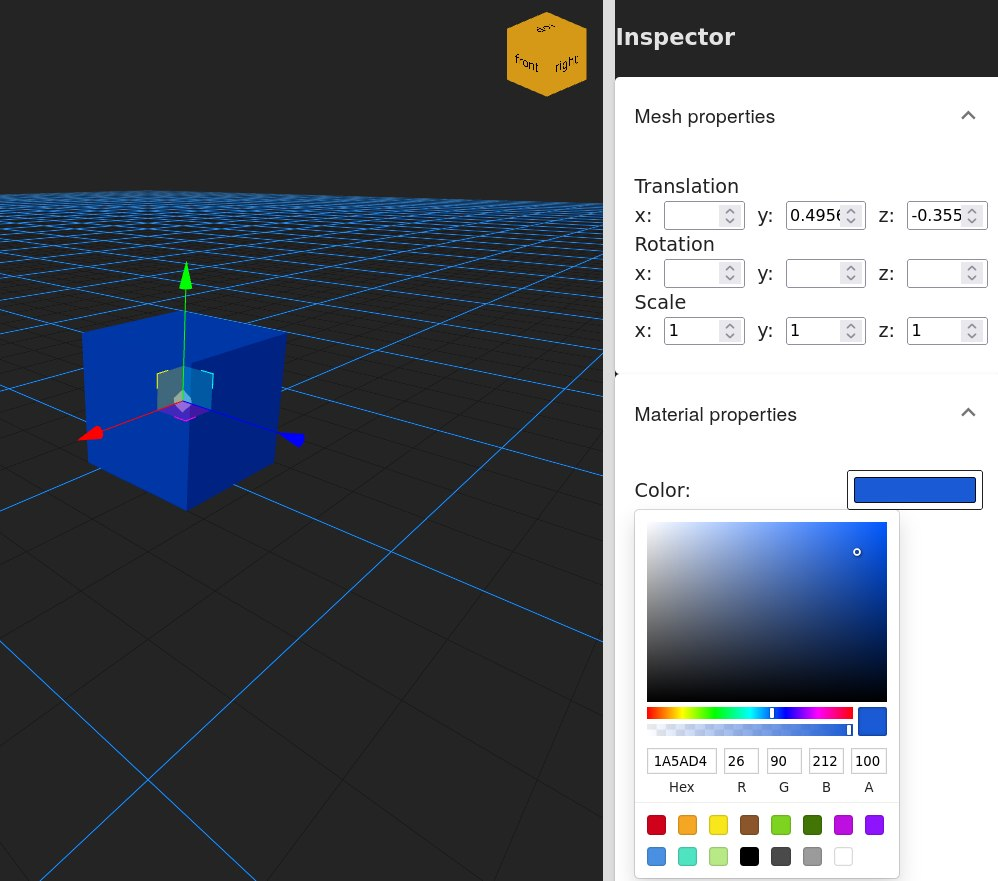
\includegraphics[width=.9\linewidth]{./img/inspector-demo.jpg}
\end{center}
\begin{itemize}
\item \sout{Integracja projektów z Azurem - Przechowywanie projektów na serwerze;}
\begin{itemize}
\item Przesunięte na etap 3/4;
\end{itemize}
\item \sout{Auto save - Automatyczne zapisywanie projektu co określony interwał czasowy;}
\begin{itemize}
\item Przesunięte na etap 4;
\end{itemize}
\item Deploy na Azure - \url{https://cadr;studio/}
\item Poprawki w UI;
\end{itemize}
\begin{center}
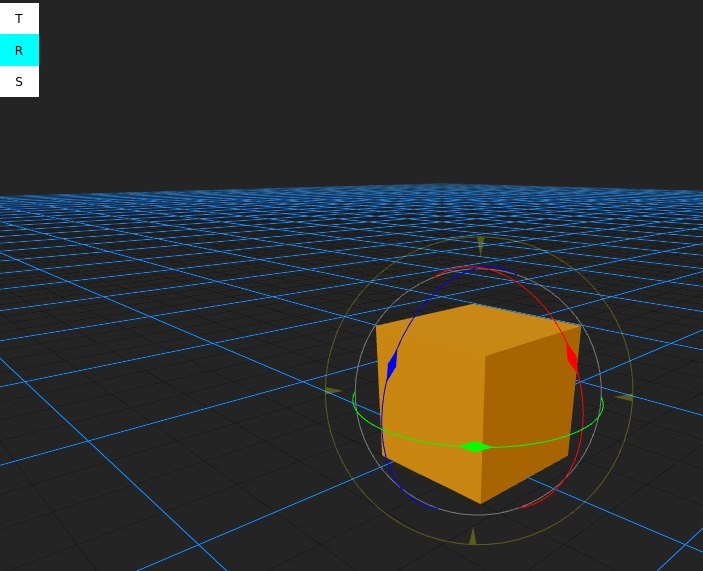
\includegraphics[width=.9\linewidth]{./img/toolbar.jpg}
\end{center}
\begin{center}
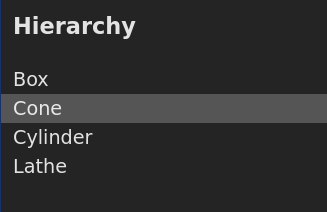
\includegraphics[width=.9\linewidth]{./img/hierarchy.jpg}
\end{center}
\subsection{Backend}
\label{sec:orge73d031}
\begin{itemize}
\item \sout{Zapisywanie projektów 1/2;}
\begin{itemize}
\item Przesunięte na etap 3;
\end{itemize}
\item Deploy na Azure -  \url{https://cadr-api.azurewebsites.net/docs/}
\item Usprawnienie refresh tokenów;
\end{itemize}
\section{Etap 3.}
\label{sec:orgcfb40e8}
\subsection{Frontend}
\label{sec:org94cdbe6}
\begin{itemize}
\item \sout{Kolaboracja w czasie rzeczywistym;}
\begin{itemize}
\item Przesunięte jako plan na przyszłość;
\end{itemize}
\item \sout{Okno projektowe - Umożliwa zapisanie i ładowanie tekstur, shaderów;}
\begin{itemize}
\item Przesunięte jako plan na przyszłość;
\end{itemize}
\item \sout{Inspektor c.d;}
\begin{itemize}
\item Przesunięte na etap 4;
\end{itemize}
\item Wsparcie dla klawiatury;
\item Import/eksport projektów;
\item Import modeli 1/2;
\end{itemize}
\begin{center}
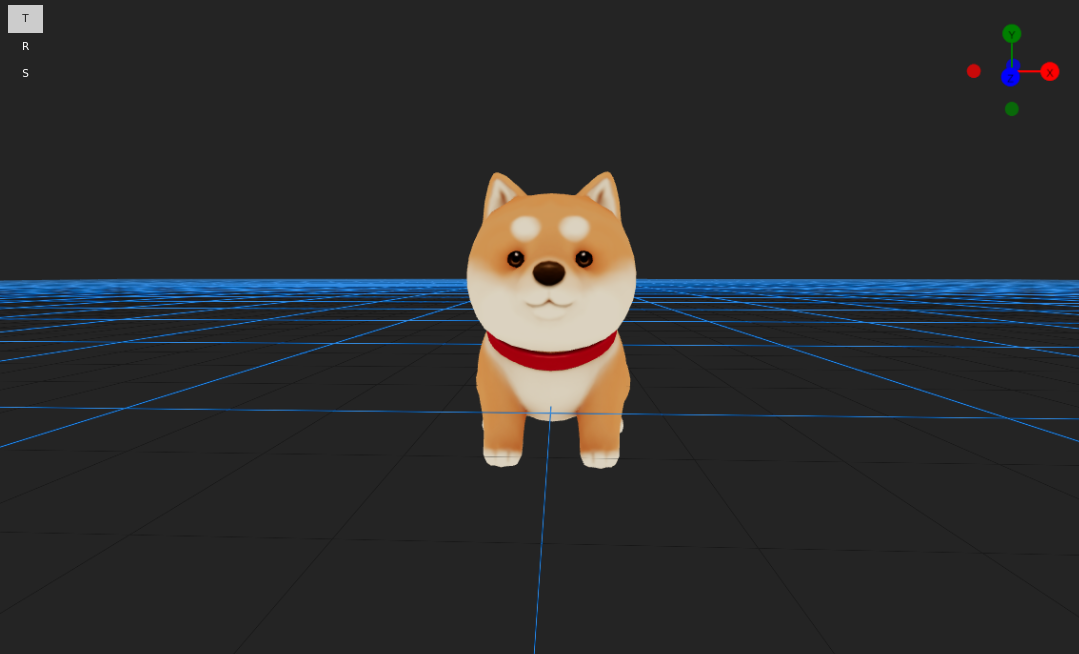
\includegraphics[width=.9\linewidth]{./img/model.jpg}
\end{center}
\begin{itemize}
\item Lepsze gizmo orientacyjne;
\end{itemize}
\begin{center}
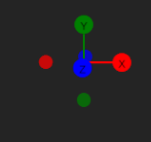
\includegraphics[width=.9\linewidth]{./img/gizmo.jpg}
\end{center}
\begin{itemize}
\item Poprawki w UI;
\end{itemize}
\subsection{Backend}
\label{sec:orgc692a91}
\begin{itemize}
\item Zapisywanie projektów 1/2;
\item \sout{Komunikacja websocket;}
\begin{itemize}
\item Przesunięte jako plan na przyszłość;
\end{itemize}
\end{itemize}
\section{Etap 4.}
\label{sec:org4458288}
\subsection{Frontend}
\label{sec:org2f5443c}
\begin{itemize}
\item Testy;
\item Funkcja automatycznego zapisywania co określony interwał czasowy;
\item Wyświetlanie zapisanych projektów;
\item Różne typy oświetlenia;
\item Inspektor;
\item Import modeli 1/2;
\end{itemize}
\subsection{Backend}
\label{sec:org91d7526}
\begin{itemize}
\item Testy end-2-end;
\item Zapisywanie projektów;
\end{itemize}
\end{document}
